\documentclass[12pt]{article}
\usepackage[utf8]{inputenc}
\usepackage{pgf,tikz,pgfplots}
\pgfplotsset{compat=1.15}
\usepackage{mathrsfs}
\usetikzlibrary{arrows}
\usepackage{fontspec}
\setmainfont[Renderer=ICU,Mapping=tex-text]{Cousine}
\usepackage{amssymb}
\usepackage[paperwidth=138.7cm,paperheight=58.0cm,left=0.1cm,right=0.1cm,top=0.1cm,bottom=0.1cm]{geometry}
\begin{document}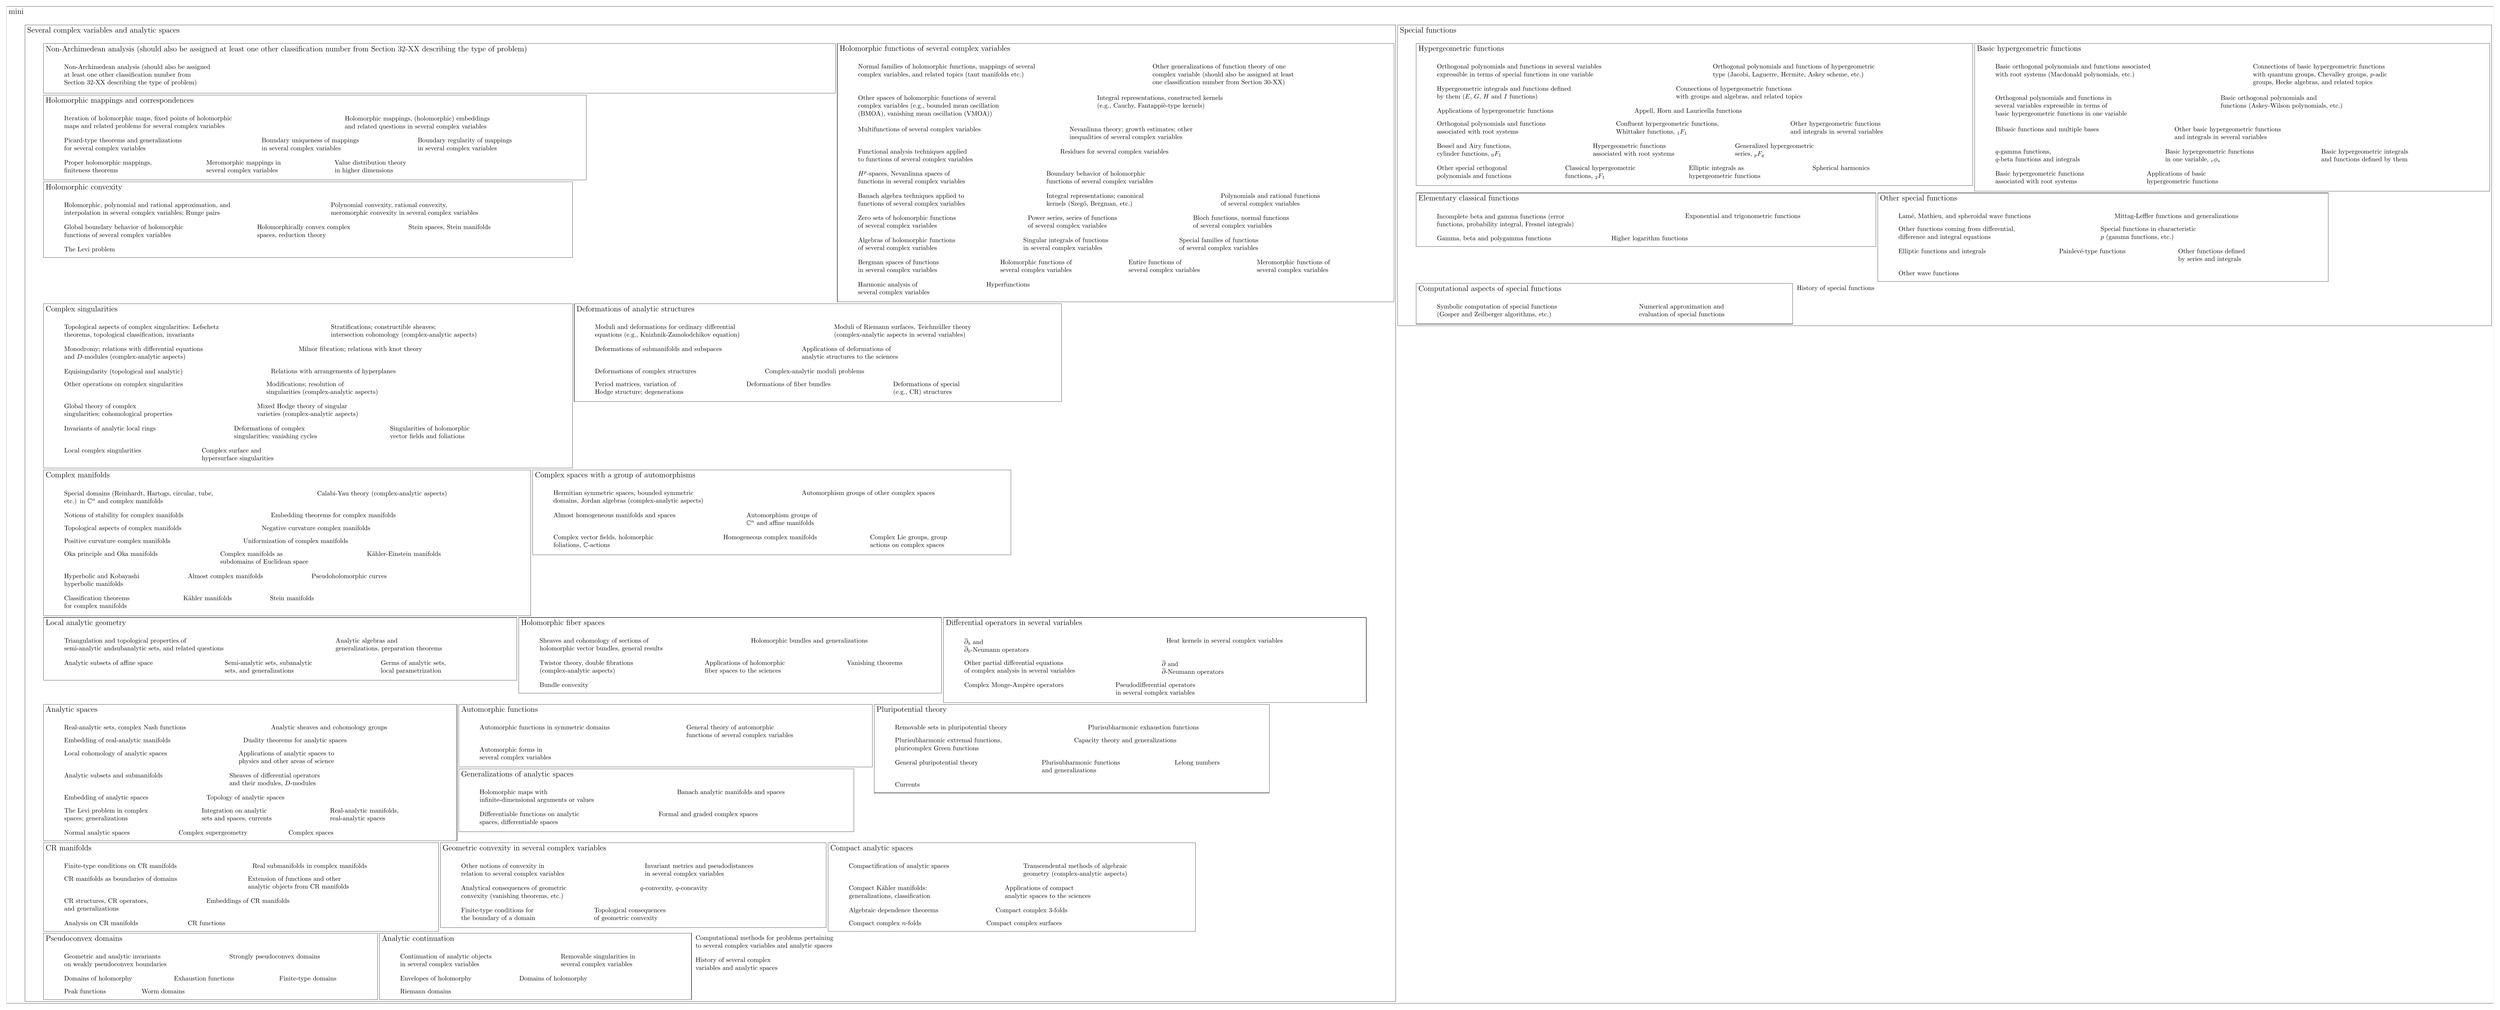
\begin{tikzpicture}[line cap=round,line join=round,>=triangle 45,x=1cm,y=1cm]
\clip(0, 0)rectangle(134.7, -54.0);

\draw(0, 0) node[anchor=north west] { \large mini};
\draw (0, 0) rectangle (134.7,-54.0);
\draw(1, -1) node[anchor=north west] { \large Several complex variables and analytic spaces};
\draw (1, -1) rectangle (75.25,-53.9);
\draw(2, -2) node[anchor=north west] { \large Non-Archimedean analysis (should also be assigned at least one other classification number from Section 32-XX describing the type of problem)};
\draw (2, -2) rectangle (44.9,-4.7);
\draw(3, -3) node[anchor=north west,align=left] {Non-Archimedean analysis (should also be assigned\\ at least one other classification number from\\ Section 32-XX describing the type of problem)};

\draw(45.0, -2) node[anchor=north west] { \large Holomorphic functions of several complex variables};
\draw (45.0, -2) rectangle (75.15,-15.999999999999996);
\draw(46.0, -3) node[anchor=north west,align=left] {Normal families of holomorphic functions, mappings of several\\ complex variables, and related topics (taut manifolds etc.)};

\draw(61.95, -3) node[anchor=north west,align=left] {Other generalizations of function theory of one\\ complex variable (should also be assigned at least\\ one classification number from Section 30-XX)};

\draw(46.0, -4.7) node[anchor=north west,align=left] {Other spaces of holomorphic functions of several\\ complex variables (e.g., bounded mean oscillation\\ (BMOA), vanishing mean oscillation (VMOA))};

\draw(58.95, -4.7) node[anchor=north west,align=left] {Integral representations, constructed kernels\\ (e.g., Cauchy, Fantappiè-type kernels)};

\draw(46.0, -6.4) node[anchor=north west,align=left] {Multifunctions of several complex variables};

\draw(57.45, -6.4) node[anchor=north west,align=left] {Nevanlinna theory; growth estimates; other\\ inequalities of several complex variables};

\draw(46.0, -7.6000000000000005) node[anchor=north west,align=left] {Functional analysis techniques applied \\ to functions of several complex variables};

\draw(56.95, -7.6000000000000005) node[anchor=north west,align=left] {Residues for several complex variables};

\draw(46.0, -8.8) node[anchor=north west,align=left] {\(H^p\)-spaces, Nevanlinna spaces of\\ functions in several complex variables};

\draw(56.2, -8.8) node[anchor=north west,align=left] {Boundary behavior of holomorphic \\ functions of several complex variables};

\draw(46.0, -10.0) node[anchor=north west,align=left] {Banach algebra techniques applied to\\ functions of several complex variables};

\draw(56.2, -10.0) node[anchor=north west,align=left] {Integral representations; canonical\\ kernels (Szegő, Bergman, etc.)};

\draw(65.65, -10.0) node[anchor=north west,align=left] {Polynomials and rational functions\\ of several complex variables};

\draw(46.0, -11.2) node[anchor=north west,align=left] {Zero sets of holomorphic functions\\ of several complex variables};

\draw(55.2, -11.2) node[anchor=north west,align=left] {Power series, series of functions\\ of several complex variables};

\draw(64.15, -11.2) node[anchor=north west,align=left] {Bloch functions, normal functions\\ of several complex variables};

\draw(46.0, -12.399999999999999) node[anchor=north west,align=left] {Algebras of holomorphic functions\\ of several complex variables};

\draw(54.95, -12.399999999999999) node[anchor=north west,align=left] {Singular integrals of functions\\ in several complex variables};

\draw(63.4, -12.399999999999999) node[anchor=north west,align=left] {Special families of functions\\ of several complex variables};

\draw(46.0, -13.599999999999998) node[anchor=north west,align=left] {Bergman spaces of functions\\ in several complex variables};

\draw(53.7, -13.599999999999998) node[anchor=north west,align=left] {Holomorphic functions of\\ several complex variables};

\draw(60.65, -13.599999999999998) node[anchor=north west,align=left] {Entire functions of \\ several complex variables};

\draw(67.6, -13.599999999999998) node[anchor=north west,align=left] {Meromorphic functions of\\ several complex variables};

\draw(46.0, -14.799999999999997) node[anchor=north west,align=left] {Harmonic analysis of \\ several complex variables};

\draw(52.95, -14.799999999999997) node[anchor=north west,align=left] {Hyperfunctions};

\draw(2, -4.800000000000001) node[anchor=north west] { \large Holomorphic mappings and correspondences};
\draw (2, -4.800000000000001) rectangle (31.400000000000006,-9.4);
\draw(3, -5.800000000000001) node[anchor=north west,align=left] {Iteration of holomorphic maps, fixed points of holomorphic\\ maps and related problems for several complex variables};

\draw(18.200000000000003, -5.800000000000001) node[anchor=north west,align=left] {Holomorphic mappings, (holomorphic) embeddings \\ and related questions in several complex variables};

\draw(3, -7.000000000000001) node[anchor=north west,align=left] {Picard-type theorems and generalizations\\ for several complex variables};

\draw(13.7, -7.000000000000001) node[anchor=north west,align=left] {Boundary uniqueness of mappings\\ in several complex variables};

\draw(22.15, -7.000000000000001) node[anchor=north west,align=left] {Boundary regularity of mappings\\ in several complex variables};

\draw(3, -8.200000000000001) node[anchor=north west,align=left] {Proper holomorphic mappings,\\ finiteness theorems};

\draw(10.7, -8.200000000000001) node[anchor=north west,align=left] {Meromorphic mappings in\\ several complex variables};

\draw(17.65, -8.200000000000001) node[anchor=north west,align=left] {Value distribution theory\\ in higher dimensions};

\draw(2, -9.499999999999998) node[anchor=north west] { \large Holomorphic convexity};
\draw (2, -9.499999999999998) rectangle (30.65,-13.599999999999998);
\draw(3, -10.499999999999998) node[anchor=north west,align=left] {Holomorphic, polynomial and rational approximation, and\\ interpolation in several complex variables; Runge pairs};

\draw(17.45, -10.499999999999998) node[anchor=north west,align=left] {Polynomial convexity, rational convexity, \\ meromorphic convexity in several complex variables};

\draw(3, -11.7) node[anchor=north west,align=left] {Global boundary behavior of holomorphic\\ functions of several complex variables};

\draw(13.45, -11.7) node[anchor=north west,align=left] {Holomorphically convex complex\\ spaces, reduction theory};

\draw(21.65, -11.7) node[anchor=north west,align=left] {Stein spaces, Stein manifolds};

\draw(3, -12.899999999999999) node[anchor=north west,align=left] {The Levi problem};

\draw(2, -16.099999999999994) node[anchor=north west] { \large Complex singularities};
\draw (2, -16.099999999999994) rectangle (30.65,-24.999999999999993);
\draw(3, -17.099999999999994) node[anchor=north west,align=left] {Topological aspects of complex singularities: Lefschetz\\ theorems, topological classification, invariants};

\draw(17.45, -17.099999999999994) node[anchor=north west,align=left] {Stratifications; constructible sheaves; \\ intersection cohomology (complex-analytic aspects)};

\draw(3, -18.299999999999994) node[anchor=north west,align=left] {Monodromy; relations with differential equations\\ and \(D\)-modules (complex-analytic aspects)};

\draw(15.7, -18.299999999999994) node[anchor=north west,align=left] {Milnor fibration; relations with knot theory};

\draw(3, -19.499999999999993) node[anchor=north west,align=left] {Equisingularity (topological and analytic)};

\draw(14.2, -19.499999999999993) node[anchor=north west,align=left] {Relations with arrangements of hyperplanes};

\draw(3, -20.199999999999996) node[anchor=north west,align=left] {Other operations on complex singularities};

\draw(13.95, -20.199999999999996) node[anchor=north west,align=left] {Modifications; resolution of \\ singularities (complex-analytic aspects)};

\draw(3, -21.399999999999995) node[anchor=north west,align=left] {Global theory of complex \\ singularities; cohomological properties};

\draw(13.45, -21.399999999999995) node[anchor=north west,align=left] {Mixed Hodge theory of singular \\ varieties (complex-analytic aspects)};

\draw(3, -22.599999999999994) node[anchor=north west,align=left] {Invariants of analytic local rings};

\draw(12.2, -22.599999999999994) node[anchor=north west,align=left] {Deformations of complex \\ singularities; vanishing cycles};

\draw(20.65, -22.599999999999994) node[anchor=north west,align=left] {Singularities of holomorphic\\ vector fields and foliations};

\draw(3, -23.799999999999997) node[anchor=north west,align=left] {Local complex singularities};

\draw(10.45, -23.799999999999997) node[anchor=north west,align=left] {Complex surface and \\ hypersurface singularities};

\draw(30.75, -16.099999999999994) node[anchor=north west] { \large Deformations of analytic structures};
\draw (30.75, -16.099999999999994) rectangle (57.15,-21.399999999999995);
\draw(31.75, -17.099999999999994) node[anchor=north west,align=left] {Moduli and deformations for ordinary differential\\ equations (e.g., Knizhnik-Zamolodchikov equation)};

\draw(44.7, -17.099999999999994) node[anchor=north west,align=left] {Moduli of Riemann surfaces, Teichmüller theory\\ (complex-analytic aspects in several variables)};

\draw(31.75, -18.299999999999994) node[anchor=north west,align=left] {Deformations of submanifolds and subspaces};

\draw(42.95, -18.299999999999994) node[anchor=north west,align=left] {Applications of deformations of \\ analytic structures to the sciences};

\draw(31.75, -19.499999999999993) node[anchor=north west,align=left] {Deformations of complex structures};

\draw(40.95, -19.499999999999993) node[anchor=north west,align=left] {Complex-analytic moduli problems};

\draw(31.75, -20.199999999999996) node[anchor=north west,align=left] {Period matrices, variation of\\ Hodge structure; degenerations};

\draw(39.95, -20.199999999999996) node[anchor=north west,align=left] {Deformations of fiber bundles};

\draw(47.9, -20.199999999999996) node[anchor=north west,align=left] {Deformations of special\\ (e.g., CR) structures};

\draw(2, -25.099999999999994) node[anchor=north west] { \large Complex manifolds};
\draw (2, -25.099999999999994) rectangle (28.4,-32.99999999999999);
\draw(3, -26.099999999999994) node[anchor=north west,align=left] {Special domains (Reinhardt, Hartogs, circular, tube,\\ etc.) in \(\mathbb{C}^n\) and complex manifolds};

\draw(16.7, -26.099999999999994) node[anchor=north west,align=left] {Calabi-Yau theory (complex-analytic aspects)};

\draw(3, -27.299999999999994) node[anchor=north west,align=left] {Notions of stability for complex manifolds};

\draw(14.2, -27.299999999999994) node[anchor=north west,align=left] {Embedding theorems for complex manifolds};

\draw(3, -27.999999999999993) node[anchor=north west,align=left] {Topological aspects of complex manifolds};

\draw(13.7, -27.999999999999993) node[anchor=north west,align=left] {Negative curvature complex manifolds};

\draw(3, -28.699999999999996) node[anchor=north west,align=left] {Positive curvature complex manifolds};

\draw(12.7, -28.699999999999996) node[anchor=north west,align=left] {Uniformization of complex manifolds};

\draw(3, -29.399999999999995) node[anchor=north west,align=left] {Oka principle and Oka manifolds};

\draw(11.45, -29.399999999999995) node[anchor=north west,align=left] {Complex manifolds as \\ subdomains of Euclidean space};

\draw(19.4, -29.399999999999995) node[anchor=north west,align=left] {Kähler-Einstein manifolds};

\draw(3, -30.599999999999994) node[anchor=north west,align=left] {Hyperbolic and Kobayashi\\ hyperbolic manifolds};

\draw(9.7, -30.599999999999994) node[anchor=north west,align=left] {Almost complex manifolds};

\draw(16.4, -30.599999999999994) node[anchor=north west,align=left] {Pseudoholomorphic curves};

\draw(3, -31.799999999999997) node[anchor=north west,align=left] {Classification theorems\\ for complex manifolds};

\draw(9.45, -31.799999999999997) node[anchor=north west,align=left] {Kähler manifolds};

\draw(14.149999999999999, -31.799999999999997) node[anchor=north west,align=left] {Stein manifolds};

\draw(28.5, -25.099999999999994) node[anchor=north west] { \large Complex spaces with a group of automorphisms};
\draw (28.5, -25.099999999999994) rectangle (54.4,-29.699999999999996);
\draw(29.5, -26.099999999999994) node[anchor=north west,align=left] {Hermitian symmetric spaces, bounded symmetric \\ domains, Jordan algebras (complex-analytic aspects)};

\draw(42.95, -26.099999999999994) node[anchor=north west,align=left] {Automorphism groups of other complex spaces};

\draw(29.5, -27.299999999999994) node[anchor=north west,align=left] {Almost homogeneous manifolds and spaces};

\draw(39.95, -27.299999999999994) node[anchor=north west,align=left] {Automorphism groups of \\ \(\mathbb{C}^n\) and affine manifolds};

\draw(29.5, -28.499999999999993) node[anchor=north west,align=left] {Complex vector fields, holomorphic\\ foliations, \(\mathbb{C}\)-actions};

\draw(38.7, -28.499999999999993) node[anchor=north west,align=left] {Homogeneous complex manifolds};

\draw(46.65, -28.499999999999993) node[anchor=north west,align=left] {Complex Lie groups, group\\ actions on complex spaces};

\draw(2, -33.099999999999994) node[anchor=north west] { \large Local analytic geometry};
\draw (2, -33.099999999999994) rectangle (27.65,-36.49999999999999);
\draw(3, -34.099999999999994) node[anchor=north west,align=left] {Triangulation and topological properties of \\ semi-analytic andsubanalytic sets, and related questions};

\draw(17.7, -34.099999999999994) node[anchor=north west,align=left] {Analytic algebras and \\ generalizations, preparation theorems};

\draw(3, -35.3) node[anchor=north west,align=left] {Analytic subsets of affine space};

\draw(11.7, -35.3) node[anchor=north west,align=left] {Semi-analytic sets, subanalytic\\ sets, and generalizations};

\draw(20.15, -35.3) node[anchor=north west,align=left] {Germs of analytic sets,\\ local parametrization};

\draw(27.75, -33.099999999999994) node[anchor=north west] { \large Holomorphic fiber spaces};
\draw (27.75, -33.099999999999994) rectangle (50.65,-37.199999999999996);
\draw(28.75, -34.099999999999994) node[anchor=north west,align=left] {Sheaves and cohomology of sections of \\ holomorphic vector bundles, general results};

\draw(40.2, -34.099999999999994) node[anchor=north west,align=left] {Holomorphic bundles and generalizations};

\draw(28.75, -35.3) node[anchor=north west,align=left] {Twistor theory, double fibrations\\ (complex-analytic aspects)};

\draw(37.7, -35.3) node[anchor=north west,align=left] {Applications of holomorphic\\ fiber spaces to the sciences};

\draw(45.4, -35.3) node[anchor=north west,align=left] {Vanishing theorems};

\draw(28.75, -36.49999999999999) node[anchor=north west,align=left] {Bundle convexity};

\draw(50.75, -33.099999999999994) node[anchor=north west] { \large Differential operators in several variables};
\draw (50.75, -33.099999999999994) rectangle (73.65,-37.699999999999996);
\draw(51.75, -34.099999999999994) node[anchor=north west,align=left] {\(\overline\partial_b\) and \\ \(\overline\partial_b\)-Neumann operators};

\draw(62.7, -34.099999999999994) node[anchor=north west,align=left] {Heat kernels in several complex variables};

\draw(51.75, -35.3) node[anchor=north west,align=left] {Other partial differential equations \\ of complex analysis in several variables};

\draw(62.45, -35.3) node[anchor=north west,align=left] {\(\overline\partial\) and \\ \(\overline\partial\)-Neumann operators};

\draw(51.75, -36.49999999999999) node[anchor=north west,align=left] {Complex Monge-Ampère operators};

\draw(59.95, -36.49999999999999) node[anchor=north west,align=left] {Pseudodifferential operators\\ in several complex variables};

\draw(2, -37.8) node[anchor=north west] { \large Analytic spaces};
\draw (2, -37.8) rectangle (24.4,-45.199999999999996);
\draw(3, -38.8) node[anchor=north west,align=left] {Real-analytic sets, complex Nash functions};

\draw(14.2, -38.8) node[anchor=north west,align=left] {Analytic sheaves and cohomology groups};

\draw(3, -39.5) node[anchor=north west,align=left] {Embedding of real-analytic manifolds};

\draw(12.7, -39.5) node[anchor=north west,align=left] {Duality theorems for analytic spaces};

\draw(3, -40.199999999999996) node[anchor=north west,align=left] {Local cohomology of analytic spaces};

\draw(12.45, -40.199999999999996) node[anchor=north west,align=left] {Applications of analytic spaces to\\ physics and other areas of science};

\draw(3, -41.4) node[anchor=north west,align=left] {Analytic subsets and submanifolds};

\draw(11.95, -41.4) node[anchor=north west,align=left] {Sheaves of differential operators\\ and their modules, \(D\)-modules};

\draw(3, -42.599999999999994) node[anchor=north west,align=left] {Embedding of analytic spaces};

\draw(10.7, -42.599999999999994) node[anchor=north west,align=left] {Topology of analytic spaces};

\draw(3, -43.3) node[anchor=north west,align=left] {The Levi problem in complex\\ spaces; generalizations};

\draw(10.45, -43.3) node[anchor=north west,align=left] {Integration on analytic\\ sets and spaces, currents};

\draw(17.4, -43.3) node[anchor=north west,align=left] {Real-analytic manifolds,\\ real-analytic spaces};

\draw(3, -44.5) node[anchor=north west,align=left] {Normal analytic spaces};

\draw(9.2, -44.5) node[anchor=north west,align=left] {Complex supergeometry};

\draw(15.149999999999999, -44.5) node[anchor=north west,align=left] {Complex spaces};

\draw(24.5, -37.8) node[anchor=north west] { \large Automorphic functions};
\draw (24.5, -37.8) rectangle (46.9,-41.199999999999996);
\draw(25.5, -38.8) node[anchor=north west,align=left] {Automorphic functions in symmetric domains};

\draw(36.7, -38.8) node[anchor=north west,align=left] {General theory of automorphic \\ functions of several complex variables};

\draw(25.5, -40.0) node[anchor=north west,align=left] {Automorphic forms in \\ several complex variables};

\draw(24.5, -41.3) node[anchor=north west] { \large Generalizations of analytic spaces};
\draw (24.5, -41.3) rectangle (45.9,-44.699999999999996);
\draw(25.5, -42.3) node[anchor=north west,align=left] {Holomorphic maps with \\ infinite-dimensional arguments or values};

\draw(36.2, -42.3) node[anchor=north west,align=left] {Banach analytic manifolds and spaces};

\draw(25.5, -43.5) node[anchor=north west,align=left] {Differentiable functions on analytic\\ spaces, differentiable spaces};

\draw(35.2, -43.5) node[anchor=north west,align=left] {Formal and graded complex spaces};

\draw(47.0, -37.8) node[anchor=north west] { \large Pluripotential theory};
\draw (47.0, -37.8) rectangle (68.4,-42.599999999999994);
\draw(48.0, -38.8) node[anchor=north west,align=left] {Removable sets in pluripotential theory};

\draw(58.45, -38.8) node[anchor=north west,align=left] {Plurisubharmonic exhaustion functions};

\draw(48.0, -39.5) node[anchor=north west,align=left] {Plurisubharmonic extremal functions,\\ pluricomplex Green functions};

\draw(57.7, -39.5) node[anchor=north west,align=left] {Capacity theory and generalizations};

\draw(48.0, -40.699999999999996) node[anchor=north west,align=left] {General pluripotential theory};

\draw(55.95, -40.699999999999996) node[anchor=north west,align=left] {Plurisubharmonic functions\\ and generalizations};

\draw(63.15, -40.699999999999996) node[anchor=north west,align=left] {Lelong numbers};

\draw(48.0, -41.9) node[anchor=north west,align=left] {Currents};

\draw(2, -45.3) node[anchor=north west] { \large CR manifolds};
\draw (2, -45.3) rectangle (23.4,-50.099999999999994);
\draw(3, -46.3) node[anchor=north west,align=left] {Finite-type conditions on CR manifolds};

\draw(13.2, -46.3) node[anchor=north west,align=left] {Real submanifolds in complex manifolds};

\draw(3, -47.0) node[anchor=north west,align=left] {CR manifolds as boundaries of domains};

\draw(12.95, -47.0) node[anchor=north west,align=left] {Extension of functions and other\\ analytic objects from CR manifolds};

\draw(3, -48.199999999999996) node[anchor=north west,align=left] {CR structures, CR operators,\\ and generalizations};

\draw(10.7, -48.199999999999996) node[anchor=north west,align=left] {Embeddings of CR manifolds};

\draw(3, -49.4) node[anchor=north west,align=left] {Analysis on CR manifolds};

\draw(9.7, -49.4) node[anchor=north west,align=left] {CR functions};

\draw(23.5, -45.3) node[anchor=north west] { \large Geometric convexity in several complex variables};
\draw (23.5, -45.3) rectangle (44.4,-49.9);
\draw(24.5, -46.3) node[anchor=north west,align=left] {Other notions of convexity in \\ relation to several complex variables};

\draw(34.45, -46.3) node[anchor=north west,align=left] {Invariant metrics and pseudodistances\\ in several complex variables};

\draw(24.5, -47.5) node[anchor=north west,align=left] {Analytical consequences of geometric\\ convexity (vanishing theorems, etc.)};

\draw(34.2, -47.5) node[anchor=north west,align=left] {\(q\)-convexity, \(q\)-concavity};

\draw(24.5, -48.699999999999996) node[anchor=north west,align=left] {Finite-type conditions for\\ the boundary of a domain};

\draw(31.7, -48.699999999999996) node[anchor=north west,align=left] {Topological consequences\\ of geometric convexity};

\draw(44.5, -45.3) node[anchor=north west] { \large Compact analytic spaces};
\draw (44.5, -45.3) rectangle (64.4,-50.099999999999994);
\draw(45.5, -46.3) node[anchor=north west,align=left] {Compactification of analytic spaces};

\draw(54.95, -46.3) node[anchor=north west,align=left] {Transcendental methods of algebraic\\ geometry (complex-analytic aspects)};

\draw(45.5, -47.5) node[anchor=north west,align=left] {Compact Kähler manifolds: \\ generalizations, classification};

\draw(53.95, -47.5) node[anchor=north west,align=left] {Applications of compact \\ analytic spaces to the sciences};

\draw(45.5, -48.699999999999996) node[anchor=north west,align=left] {Algebraic dependence theorems};

\draw(53.45, -48.699999999999996) node[anchor=north west,align=left] {Compact complex \(3\)-folds};

\draw(45.5, -49.4) node[anchor=north west,align=left] {Compact complex \(n\)-folds};

\draw(52.95, -49.4) node[anchor=north west,align=left] {Compact complex surfaces};

\draw(2, -50.199999999999996) node[anchor=north west] { \large Pseudoconvex domains};
\draw (2, -50.199999999999996) rectangle (20.1,-53.8);
\draw(3, -51.199999999999996) node[anchor=north west,align=left] {Geometric and analytic invariants\\ on weakly pseudoconvex boundaries};

\draw(11.95, -51.199999999999996) node[anchor=north west,align=left] {Strongly pseudoconvex domains};

\draw(3, -52.4) node[anchor=north west,align=left] {Domains of holomorphy};

\draw(8.95, -52.4) node[anchor=north west,align=left] {Exhaustion functions};

\draw(14.649999999999999, -52.4) node[anchor=north west,align=left] {Finite-type domains};

\draw(3, -53.099999999999994) node[anchor=north west,align=left] {Peak functions};

\draw(7.199999999999999, -53.099999999999994) node[anchor=north west,align=left] {Worm domains};

\draw(20.200000000000003, -50.199999999999996) node[anchor=north west] { \large Analytic continuation};
\draw (20.200000000000003, -50.199999999999996) rectangle (37.1,-53.8);
\draw(21.200000000000003, -51.199999999999996) node[anchor=north west,align=left] {Continuation of analytic objects\\ in several complex variables};

\draw(29.900000000000002, -51.199999999999996) node[anchor=north west,align=left] {Removable singularities in\\ several complex variables};

\draw(21.200000000000003, -52.4) node[anchor=north west,align=left] {Envelopes of holomorphy};

\draw(27.650000000000002, -52.4) node[anchor=north west,align=left] {Domains of holomorphy};

\draw(21.200000000000003, -53.099999999999994) node[anchor=north west,align=left] {Riemann domains};

\draw(37.2, -50.199999999999996) node[anchor=north west,align=left] {Computational methods for problems pertaining \\ to several complex variables and analytic spaces};

\draw(37.2, -51.4) node[anchor=north west,align=left] {History of several complex \\ variables and analytic spaces};

\draw(75.35, -1) node[anchor=north west] { \large Special functions};
\draw (75.35, -1) rectangle (134.6,-17.3);
\draw(76.35, -2) node[anchor=north west] { \large Hypergeometric functions};
\draw (76.35, -2) rectangle (106.5,-9.700000000000001);
\draw(77.35, -3) node[anchor=north west,align=left] {Orthogonal polynomials and functions in several variables\\ expressible in terms of special functions in one variable};

\draw(92.3, -3) node[anchor=north west,align=left] {Orthogonal polynomials and functions of hypergeometric\\ type (Jacobi, Laguerre, Hermite, Askey scheme, etc.)};

\draw(77.35, -4.2) node[anchor=north west,align=left] {Hypergeometric integrals and functions defined \\ by them (\(E\), \(G\), \(H\) and \(I\) functions)};

\draw(90.3, -4.2) node[anchor=north west,align=left] {Connections of hypergeometric functions \\ with groups and algebras, and related topics};

\draw(77.35, -5.4) node[anchor=north west,align=left] {Applications of hypergeometric functions};

\draw(88.05, -5.4) node[anchor=north west,align=left] {Appell, Horn and Lauricella functions};

\draw(77.35, -6.1000000000000005) node[anchor=north west,align=left] {Orthogonal polynomials and functions\\ associated with root systems};

\draw(87.05, -6.1000000000000005) node[anchor=north west,align=left] {Confluent hypergeometric functions,\\ Whittaker functions, \({}_1F_1\)};

\draw(96.5, -6.1000000000000005) node[anchor=north west,align=left] {Other hypergeometric functions \\ and integrals in several variables};

\draw(77.35, -7.300000000000001) node[anchor=north west,align=left] {Bessel and Airy functions, \\ cylinder functions, \({}_0F_1\)};

\draw(85.8, -7.300000000000001) node[anchor=north west,align=left] {Hypergeometric functions \\ associated with root systems};

\draw(93.5, -7.300000000000001) node[anchor=north west,align=left] {Generalized hypergeometric\\ series, \({}_pF_q\)};

\draw(77.35, -8.5) node[anchor=north west,align=left] {Other special orthogonal\\ polynomials and functions};

\draw(84.3, -8.5) node[anchor=north west,align=left] {Classical hypergeometric\\ functions, \({}_2F_1\)};

\draw(91.0, -8.5) node[anchor=north west,align=left] {Elliptic integrals as \\ hypergeometric functions};

\draw(97.69999999999999, -8.5) node[anchor=north west,align=left] {Spherical harmonics};

\draw(106.6, -2) node[anchor=north west] { \large Basic hypergeometric functions};
\draw (106.6, -2) rectangle (134.5,-10.0);
\draw(107.6, -3) node[anchor=north west,align=left] {Basic orthogonal polynomials and functions associated\\ with root systems (Macdonald polynomials, etc.)};

\draw(121.55, -3) node[anchor=north west,align=left] {Connections of basic hypergeometric functions\\ with quantum groups, Chevalley groups, \(p\)-adic\\ groups, Hecke algebras, and related topics};

\draw(107.6, -4.7) node[anchor=north west,align=left] {Orthogonal polynomials and functions in \\ several variables expressible in terms of \\ basic hypergeometric functions in one variable};

\draw(119.8, -4.7) node[anchor=north west,align=left] {Basic orthogonal polynomials and \\ functions (Askey-Wilson polynomials, etc.)};

\draw(107.6, -6.4) node[anchor=north west,align=left] {Bibasic functions and multiple bases};

\draw(117.3, -6.4) node[anchor=north west,align=left] {Other basic hypergeometric functions\\ and integrals in several variables};

\draw(107.6, -7.6000000000000005) node[anchor=north west,align=left] {\(q\)-gamma functions, \\ \(q\)-beta functions and integrals};

\draw(116.8, -7.6000000000000005) node[anchor=north west,align=left] {Basic hypergeometric functions\\ in one variable, \({}_r\phi_s\)};

\draw(125.25, -7.6000000000000005) node[anchor=north west,align=left] {Basic hypergeometric integrals\\ and functions defined by them};

\draw(107.6, -8.8) node[anchor=north west,align=left] {Basic hypergeometric functions\\ associated with root systems};

\draw(115.8, -8.8) node[anchor=north west,align=left] {Applications of basic \\ hypergeometric functions};

\draw(76.35, -10.1) node[anchor=north west] { \large Elementary classical functions};
\draw (76.35, -10.1) rectangle (101.25,-13.0);
\draw(77.35, -11.1) node[anchor=north west,align=left] {Incomplete beta and gamma functions (error \\ functions, probability integral, Fresnel integrals)};

\draw(90.8, -11.1) node[anchor=north west,align=left] {Exponential and trigonometric functions};

\draw(77.35, -12.3) node[anchor=north west,align=left] {Gamma, beta and polygamma functions};

\draw(86.8, -12.3) node[anchor=north west,align=left] {Higher logarithm functions};

\draw(101.35, -10.1) node[anchor=north west] { \large Other special functions};
\draw (101.35, -10.1) rectangle (125.75,-14.899999999999999);
\draw(102.35, -11.1) node[anchor=north west,align=left] {Lamé, Mathieu, and spheroidal wave functions};

\draw(114.05, -11.1) node[anchor=north west,align=left] {Mittag-Leffler functions and generalizations};

\draw(102.35, -11.799999999999999) node[anchor=north west,align=left] {Other functions coming from differential,\\ difference and integral equations};

\draw(113.3, -11.799999999999999) node[anchor=north west,align=left] {Special functions in characteristic\\ \(p\) (gamma functions, etc.)};

\draw(102.35, -13.0) node[anchor=north west,align=left] {Elliptic functions and integrals};

\draw(111.05, -13.0) node[anchor=north west,align=left] {Painlevé-type functions};

\draw(117.5, -13.0) node[anchor=north west,align=left] {Other functions defined\\ by series and integrals};

\draw(102.35, -14.2) node[anchor=north west,align=left] {Other wave functions};

\draw(76.35, -15.0) node[anchor=north west] { \large Computational aspects of special functions};
\draw (76.35, -15.0) rectangle (96.75,-17.2);
\draw(77.35, -16.0) node[anchor=north west,align=left] {Symbolic computation of special functions\\ (Gosper and Zeilberger algorithms, etc.)};

\draw(88.3, -16.0) node[anchor=north west,align=left] {Numerical approximation and \\ evaluation of special functions};

\draw(96.85, -15.0) node[anchor=north west,align=left] {History of special functions};

\end{tikzpicture}

\end{document}